%% ------------------------------------------------------------------------- %%
\chapter{Experimentos Preliminares}
\label{cap:experimentos}

Uma série de experimentos foram realizados com dois conjuntos de dados de pele de seres humanos. Os classificadores utilizados foram SVM, $k$-NN e a árvore de decisão \emph{fuzzy} proposta por \citet{cintra:13}. Outro aspecto estudado é o efeito da escolha do modelo de cores no classificador. A formação dos conjuntos de dados é detalhada na seção \ref{sec:datasets_descricao} e os resultados dos experimentos podem ser vistos nas seções \ref{sec:experimento_um}, \ref{sec:experimento_dois} e \ref{sec:experimento_tres}.

%------------------------------------------------------
\section{Conjuntos de dados} 
\label{sec:datasets_descricao}
Para os experimentos foram utilizadas duas bases de dados distintas. A primeira delas, denominada UCI neste trabalho, foi proposta por \citet{uci-skin-dataset:12} e obtida no repositório de aprendizagem de máquina da Universidade da Califórnia em Irvine \citep{lichman:13}. A base é constituída por imagens de várias texturas de pele e não pele obtidas a partir de milhares de imagens arbitrárias de faces de diferentes idades, sexo e raças \citep{pal-texas:04, feret:96}.

A UCI contém 245.057 amostras, compostas por 3 atributos que constituem o vetor de entradas $x = [x_1, x_2, x_3]$, $x \in \mathbb{R}^{d}$, sendo $d$ a dimensão do espaço, e que representam, respectivamente, os canais azul (B), verde (G) e vermelho (R) do modelo de cores RGB, além de uma quarta coluna que determina a classe a qual a amostra $x$ pertence, denotada por $y$, sendo $y \in Y$ e $Y = \{+1, -1\}$.

Em outras palavras, cada amostra é um pixel RGB com um determinado rótulo. Como tem-se os dados rotulados com exemplos de qual é a saída correta para uma dada entrada, os experimentos subsequentes são categorizados como sendo de aprendizado supervisionado \citep{mostafa:12}.

A tabela~\ref{tbl:uci_dataset} exemplifica um pequeno trecho da base de dados UCI. Vale ressaltar que do total das 245.057 amostras, 194.198 são de pixels não pele e 50.859 de pixels com diferentes tons de pele. Além disso, as imagens que foram utilizadas na extração do conjunto de dados não foi disponibilizada pelos autores.

\begin{table}[!htpb]
\centering
\begin{small}
\begin{tabular}{|c|c|c|c|} \hline
\thb{B} & \thb{G} & \thb{R}  & \thb{Classe}  \\ \hline
74	    & 85      & 123	     & 1     \\
207	    & 215     & 255      & 1     \\
74      & 82      & 122	     & 1     \\
202     & 211     & 255      & 1     \\
54      & 72      & 125      & 1     \\
\ldots  &\ldots   & \dots    &\ldots \\
166     & 164     & 116      & -1    \\
148     & 150     & 91       & -1    \\
29      & 26      & 5        & -1    \\
167     & 166	  & 115	     & -1    \\
180	    & 177	  & 133	     & -1    \\ \hline
\end{tabular}
\caption[Trecho com amostras da base de dados UCI]{Trecho com amostras da base de dados UCI. Cada uma das três primeiras colunas representam um canal do pixel do espaço de cores RGB e variam entre 0 e 255. A quarta coluna é a classe atribuída à amostra, que pode assumir +1 se for pele e -1, caso contrário. Originalmente, a classe que representa um pixel de não pele tinha valor 2, substituída por -1 para conformidade com os experimentos.}
\label{tbl:uci_dataset}
\end{small}
\end{table}

Uma vez que a dimensão do espaço do problema é $d = 3$, é possível plotar os dados para melhor interpretação dos mesmos, conforme mostra a figura~\ref{fig:dataset_uci}.
\begin{figure}[h]
    \centering
    \begin{minipage}{0.45\textwidth}
        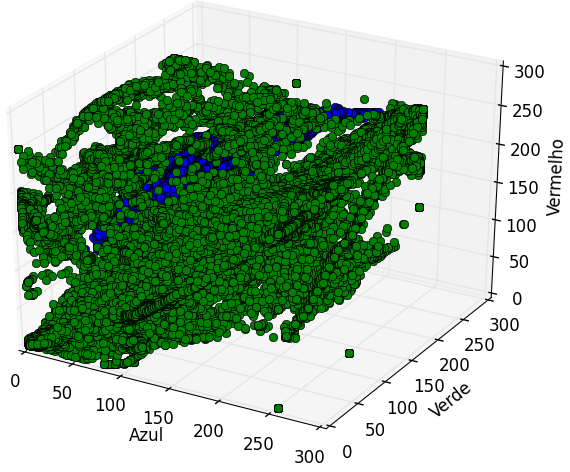
\includegraphics[width=\textwidth]{uci_skinns_plot}
    \end{minipage}
    ~ % space
    \begin{minipage}{0.45\textwidth}
        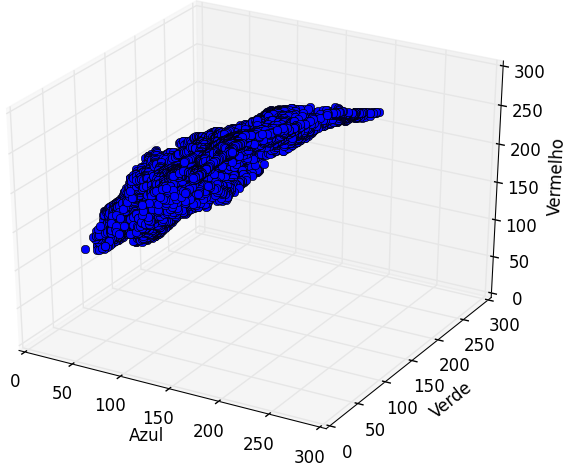
\includegraphics[width=\textwidth]{uci_skin_plot}
    \end{minipage}
    \caption[Visão 3-dimensional dos canais RGB do conjunto de dados UCI]{Visão 3-dimensional dos canais RGB do conjunto de dados UCI. Os pontos em azul são amostras de pele e os verdes de não pele. À esquerda tem-se todas as amostras do conjunto de dados; à direita apenas as amostras de pele. Fonte: proposto pelo autor.}
    \label{fig:dataset_uci}
\end{figure}

O segundo conjunto de dados utilizado nos experimentos foi proposto por \citet{sfa-skin-dataset:13}, intitulado pelos autores como banco de imagens de pele humana baseado no FERET e AR (SFA), cuja sigla também será utilizada neste trabalho. O SFA possui um conjunto de imagens de faces obtidas a partir de outros dois bancos de imagens coloridas: o FERET, criado por \citet{feret:96} e o AR, proposto por \citet{ar-face-database:98}, tendo sido utilizadas 876 e 242 imagens de cada um, respectivamente. É importante ressaltar que as imagens do AR têm fundo branco e pequenas variações de cor da pele e, portanto, o ambiente é mais controlado que as imagens do FERET \citep{sfa-skin-dataset:13}. A figura~\ref{fig:sfa_dataset_exemplo} mostra um exemplo das 1.118 imagens do banco.

\begin{figure}[h]
    \centering
    \begin{subfigure}[t]{0.21\textwidth}
        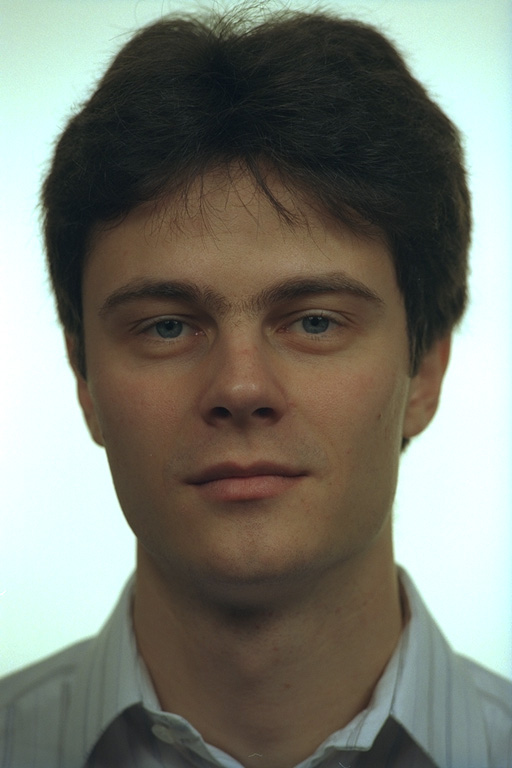
\includegraphics[width=\textwidth]{sfa_img_1}
        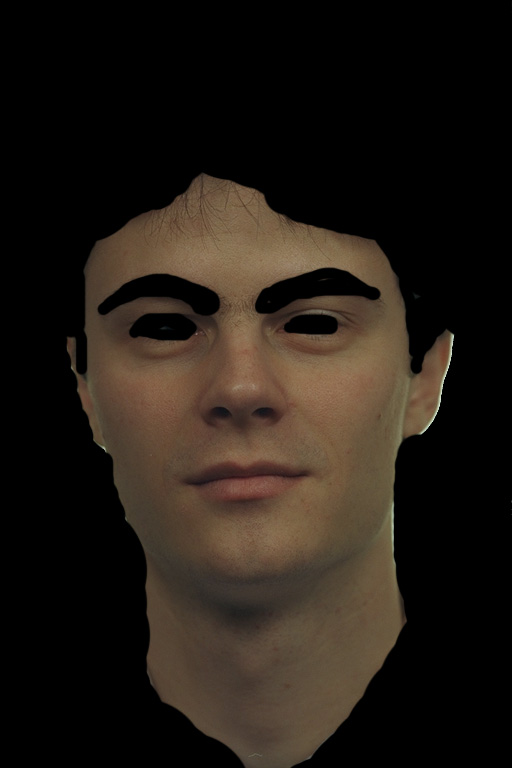
\includegraphics[width=\textwidth]{sfa_img_1_gt}
    \end{subfigure}
    ~
    \begin{subfigure}[t]{0.21\textwidth}
        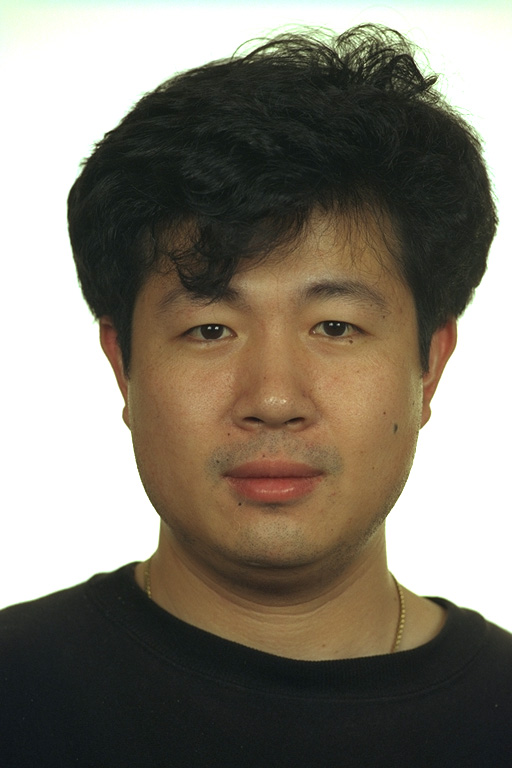
\includegraphics[width=\textwidth]{sfa_img_14}
        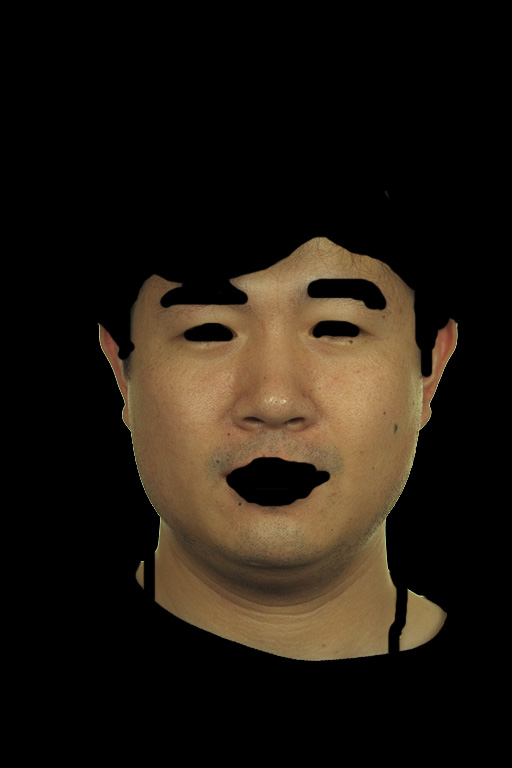
\includegraphics[width=\textwidth]{sfa_img_14_gt}
    \end{subfigure}
    ~
    \begin{subfigure}[t]{0.21\textwidth}
        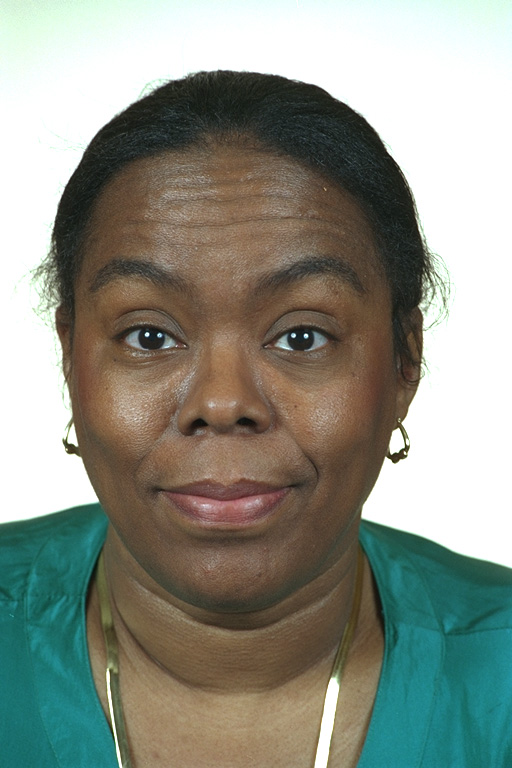
\includegraphics[width=\textwidth]{sfa_img_586}
        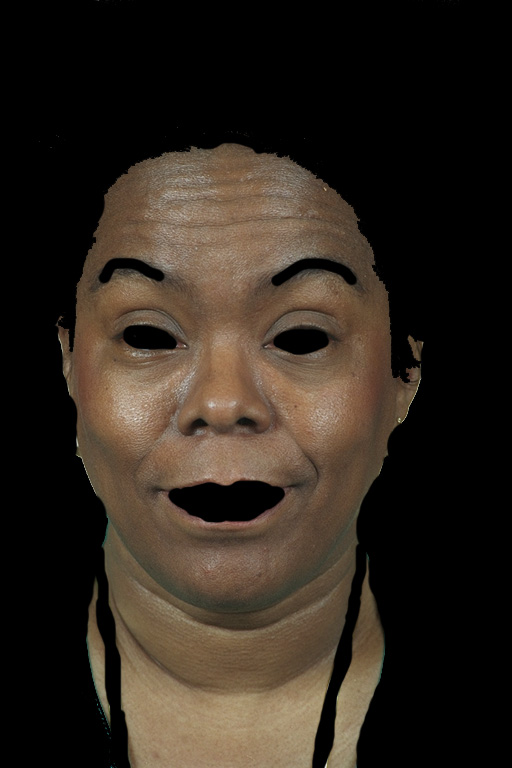
\includegraphics[width=\textwidth]{sfa_img_586_gt}
    \end{subfigure}
    ~ % space
    \begin{subfigure}[t]{0.21\textwidth}
        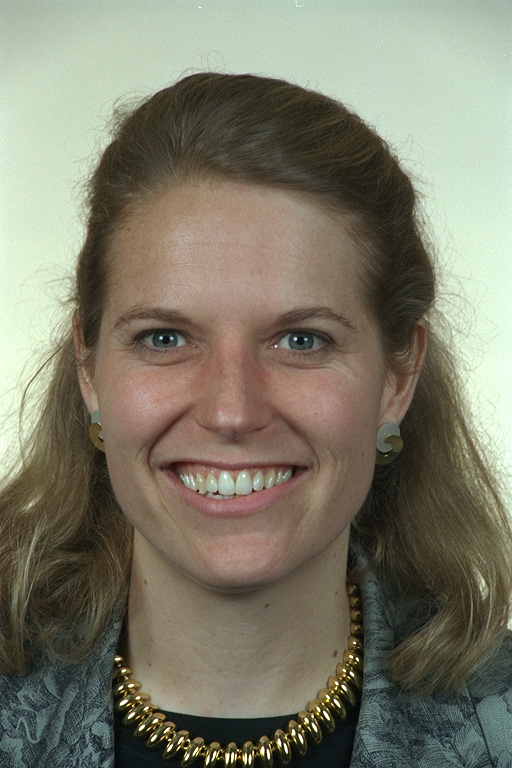
\includegraphics[width=\textwidth]{sfa_img_726}
        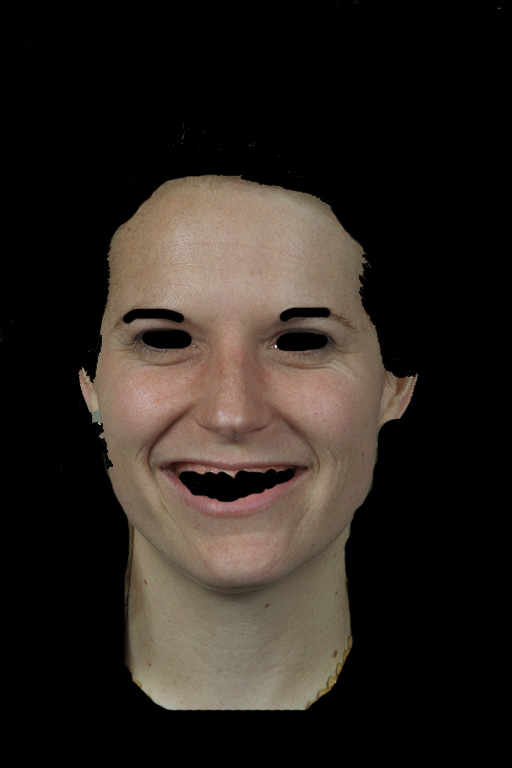
\includegraphics[width=\textwidth]{sfa_img_726_gt}
    \end{subfigure}
    \caption[Exemplos de imagens do banco de faces SFA]{Exemplos de imagens do banco de faces SFA. Na parte superior tem-se a imagem original e na inferior o ground truth com os pixels de cor de pele anotados manualmente, sendo que a cor preta RGB = (0, 0, 0) foi atribuída a todos os pixels no fundo. Fonte: \citet{sfa-skin-dataset:13}.}
    \label{fig:sfa_dataset_exemplo}
\end{figure}

As amostras de pele e não pele foram geradas aleatoriamente considerando a máscara \emph{ground truth}\footnote{\emph{Ground truth} é o termo utilizado para denotar uma imagem cujo objeto de interesse está devidamente segmentado e ressaltado, descartando os pixels remanescentes atribuindo-lhes cores uniformes.} de cada imagem, sendo três amostras de pele e cinco de não pele. Cada amostra é uma janela de tamanho $n\times n$, sendo $n$ ímpar, com um pixel central, a partir do qual outros tamanhos de amostra foram criados, que variam de $1 \times 1$ até $35 \times 35$, como pode ser visto na figura~\ref{fig:sfa_dataset_janelas} \citep{sfa-skin-dataset:13}.

\begin{figure}[h]
  \centering
  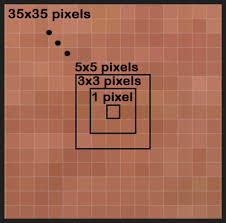
\includegraphics[width=.3\textwidth]{sfa-janelas}
  \caption[Estrutura das janelas que formam as amostras do SFA]{Estrutura das janelas que formam as amostras do SFA. No total, são 3.354 amostras de pele e outras 5.590 de não pele para cada tamanho de janela. Fonte: \citet{sfa-skin-dataset:13}.}
  \label{fig:sfa_dataset_janelas}
\end{figure}

A partir das amostras criadas no SFA, um conjunto de dados foi extraído gerando uma base de dados de pele e não pele similar ao UCI na tabela~\ref{tbl:uci_dataset}. O tamanho da janela utilizado foi $9 \times 9$ e o espaço de cores também foi o RGB. Portanto, o total de amostras empregado nos experimentos é 724.464, sendo 271.674 de pele e 452.790 de não pele. A classe atribuída à cada amostra tem o mesmo valor que no UCI, ou seja, +1 se for pele e -1, caso contrário. A figura~\ref{fig:dataset_sfa} mostra a representação gráfica dos dados plotados em 3 dimensões.
\begin{figure}[h]
    \centering
    \begin{minipage}{0.45\textwidth}
        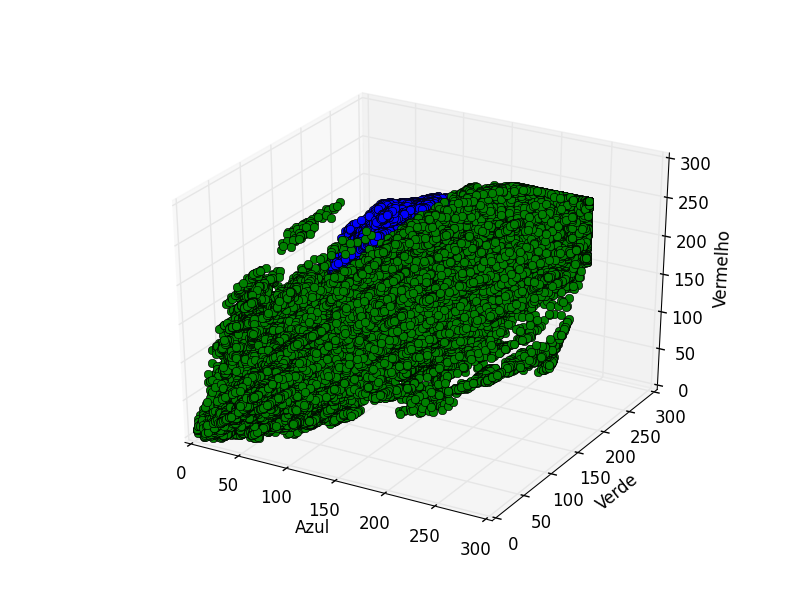
\includegraphics[width=\textwidth]{sfa_skinns_plot}
    \end{minipage}
    ~ % space
    \begin{minipage}{0.45\textwidth}
        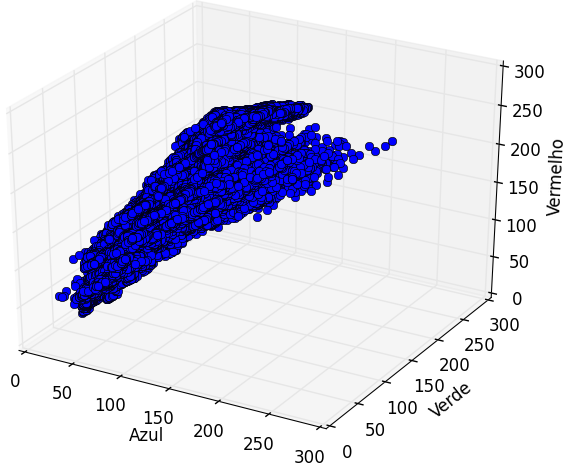
\includegraphics[width=\textwidth]{sfa_skin_plot}
    \end{minipage}
    \caption[Visão 3-dimensional dos canais RGB do conjunto de dados SFA]{Visão 3-dimensional dos canais RGB do conjunto de dados SFA. Os pontos em azul são amostras de pele e os verdes de não pele. À esquerda tem-se todas as amostras do conjunto de dados gerado; à direita apenas as amostras de pele. Fonte: proposto pelo autor.}
    \label{fig:dataset_sfa}
\end{figure}

%------------------------------------------------------
\section{Primeiro experimento}
\label{sec:experimento_um}
O primeiro experimento foi realizado com $k$-NN e SVM, disponíveis no pacote \emph{scikit-learn} \citep{scikit-learn:11}. O espaço de cores usado originalmente foi o RGB, como citado na descrição dos conjuntos de dados em \ref{sec:datasets_descricao}. Em ambos os casos, a estratégia escolhida de validação cruzada foi a \emph{10-fold}, que é uma escolha comum desta abordagem na prática \citep{mostafa:12}. Além disso, a técnica de tabela de busca\index{busca!tabela de} do \emph{scikit-learn} também foi utilizada com o objetivo de encontrar os parâmetros mais adequados para cada classificador.

A tabela de busca é usada no \emph{scikit-learn} para encontrar os parâmetros ótimos de um classificador quando eles não podem ser aprendidos pelo estimador, tais como, \emph{kernel} e $\gamma$ na SVM ou número de vizinhos no $k$-NN \citep{scikit-learn:11}. As tabelas de parâmetros utilizadas no treinamento da SVM e $k$-NN podem ser vistas em \ref{tab:svm_tabela_busca} e \ref{tab:knn_tabela_busca}. Os parâmetros de cada linha são combinados na tentativa de encontrar o estimador ótimo. Por exemplo, uma escolha no treinamento da SVM seria \emph{kernel}=rbf, C=100, \emph{gamma}=1e-4. Todas as combinações possíveis são exploradas, sendo que a melhor delas é retornada \citep{scikit-learn:11}.

\begin{table}[!htpb]
\centering
\begin{small}
\setlength{\tabcolsep}{10pt}

\begin{tabular}{|c|c|c|c|c|c|c|c|c|c|}\hline
 \thbi{kernel} & \multicolumn{4}{c|}{\thbi{C}} & \multicolumn{3}{c|}{\thbi{gamma}} & \multicolumn{2}{c|}{\thbi{degree}}\\ \cline{1-10}
rbf    & 1 & 10 & 100 & 1000 & 1e-3 & 1e-4 & 1e-5 &   &   \\ \hline
poly   & 1 & 10 & 100 & 1000 &      & 1e-4 & 1e-5 & 3 & 4 \\ \hline
linear & 1 & 10 & 100 & 1000 &      &      &      &   &   \\ \hline

\end{tabular}
\end{small}
\caption[Tabela de busca dos parâmetros do estimador ótimo na SVM]{Tabela de busca dos parâmetros do estimador ótimo na SVM. A coluna kernel refere-se aos kernels usados no treinamento que são gaussiano, polinomial e linear, respectivamente. C é um parâmetro de regularização que diz à SVM a quantidade de erro admitido no treinamento. Gamma é um parâmetro usado somente nos kernels gaussiano e polinomial, conforme citado em \ref{sec:clasificadores_svm}. Degree é o grau do polinômio; usado somente no kernel polinomial \citep{scikit-learn:11}.}
\label{tab:svm_tabela_busca}
\end{table}

\begin{table}[!htpb]
\centering
\begin{small}
\setlength{\tabcolsep}{8pt}

\begin{tabular}{|c|c|c|c|c|c|c|c|c|c|c|c|c|}\hline
 \multicolumn{10}{|c|}{\thbi{n\_neighbors}} & \multicolumn{2}{c|}{\thbi{weights}} & \multicolumn{1}{c|}{\thbi{algorithm}}\\ \cline{1-13}
3 & 5 & 9 & 15 & 25 & 50 & 100 & 200 & 400 & 800 & distance & uniform & auto \\ \hline

\end{tabular} 
\end{small}
\caption[Tabela de busca dos parâmetros do estimador ótimo no $k$-NN]{Tabela de busca dos parâmetros do estimador ótimo no k-NN. A coluna n\_neighbors refere-se ao número de vizinhos considerado no treinamento. Weights é a função peso usada na predição, onde uniform indica que os pontos têm pesos iguais e distance indica que o inverso da distância é aplicado na classificação, conforme citado em \ref{eq:knn_funcao_peso}. A terceira coluna indica qual algoritmo deve ser utiizado; auto significa que o algoritmo será decidido com base nos dados \citep{scikit-learn:11}.}
\label{tab:knn_tabela_busca}
\end{table}

Os resultados deste experimento podem ser vistos na tabela \ref{tab:resultados_experimento_um}. Vale ressaltar que o treinamento foi executado com 10 tarefas em paralelo em ambos os classificadores e 30\% dos dados, aleatoriamente, foram separados para teste.
\begin{table}[!htpb]
\centering
\begin{small}
\setlength{\tabcolsep}{8pt}

\begin{tabular}{|c|c|c|c|c|c|}\hline
 \thb{Base de dados} & \thb{Classificador} & \thb{Modelo de cores} & \thbi{Precision} & \thbi{Recall} & \thbi{F1-score} \\ \hline
 \multirow{2}{*}{UCI} & $k$-NN & RGB & 1,00 & 1,00 & 1,00 \\ \cline{2-6}
                      & SVM    & RGB & 0,98 & 0,98 & 0,98 \\ \hline
 \multirow{2}{*}{SFA} & $k$-NN & RGB & 0,9672 & 0,9669 & 0,9670 \\ \cline{2-6}
                      & SVM    & RGB & \textcolor{red}{todo} && \\ \hline

\end{tabular}
\end{small}
\caption[Resultados dos experimentos com $k$-NN e SVM nos conjuntos de dados UCI e SFA]{Resultados dos experimentos com $k$-NN e SVM nos conjuntos de dados UCI e SFA. Os parâmetros ótimos do k-NN no treinamento com UCI foram n\_neighbors=3, weights=uniform e com SFA n\_neighbors=15, weights=uniform. Os parâmetros ótimos da SVM no treinamento com UCI foram \textcolor{red}{completar}.}
\label{tab:resultados_experimento_um}
\end{table}


%------------------------------------------------------
\section{Segundo experimento}
\label{sec:experimento_dois}
Este experimento, de maneira similar ao realizado na seção \ref{sec:experimento_um}, também foi realizado com $k$-NN e SVM. Porém, o conjunto de dados SFA foi transformado para os espaços de cor HSV, Lab e YCbCr com o objetivo de compreender a influência nos resultados. Além disso, o atributo referente ao componente de luminância foi ignorado para que um teste somente com os componentes de crominância fosse realizado. Novamente, a estratégia escolhida de validação cruzada foi a \emph{10-fold}.

Os resultados podem ser vistos na tabela \ref{tab:resultados_experimento_dois}. Vale ressaltar que o treinamento foi executado com 10 tarefas em paralelo em ambos os classificadores e 30\% dos dados, aleatoriamente, foram separados para teste.
\begin{table}[!htpb]
\centering
\begin{small}
\setlength{\tabcolsep}{8pt}

\begin{tabular}{|c|c|c|c|c|}\hline
 Modelo de cores & Classificador & \emph{Precision} & \emph{Recall} & \emph{F1-score} \\ \hline
 \multirow{2}{*}{RGB}   & $k$-NN  & 0,9672 & 0,9669 & 0,9670 \\ \cline{2-5}
                        & SVM     & 0,98 & 0,98 & 0,98 \\ \hline
 \multirow{2}{*}{HSV}   & $k$-NN  & 0,9676 & 0,9673 & 0,9674 \\ \cline{2-5}
                        & SVM     & \textcolor{red}{todo} && \\ \hline
 \multirow{2}{*}{HS}    & $k$-NN  & 0,9215 & 0,9194 & 0,9199 \\ \cline{2-5}
                        & SVM     & \textcolor{red}{todo} && \\ \hline
 \multirow{2}{*}{Lab}   & $k$-NN  & 0,9671 & 0,9660 & 0,9670 \\ \cline{2-5}
                        & SVM     & \textcolor{red}{todo} && \\ \hline
 \multirow{2}{*}{ab}    & $k$-NN  & 0,9444 & 0,9439 & 0,9440 \\ \cline{2-5}
                        & SVM     & \textcolor{red}{todo} && \\ \hline
 \multirow{2}{*}{YCbCr} & $k$-NN  & 0,9679 & 0,9677 & 0,9677 \\ \cline{2-5}
                        & SVM     & \textcolor{red}{todo} && \\ \hline
 \multirow{2}{*}{CbCr}  & $k$-NN  & 0,9487 & 0,9482 & 0,9483 \\ \cline{2-5}
                        & SVM     & \textcolor{red}{todo} && \\ \hline

\end{tabular}
\end{small}
\caption[Resultados dos experimentos com $k$-NN e SVM no conjunto de dados SFA em espaços de cores distintos]{Resultados dos experimentos com $k$-NN e SVM no conjunto de dados SFA em espaços de cores distintos. As linhas com os modelos de cores HS, ab e CbCr indicam que o componente de luminância não foi utilizado no treinamento.}
\label{tab:resultados_experimento_dois}
\end{table}


%------------------------------------------------------
\section{Terceiro experimento}
\label{sec:experimento_tres}
O último experimento foi realizado com a árvore de decisão \emph{fuzzy} proposta por \citet{cintra:13}. O conjunto de dados SFA transformado para os espaços de cor HSV, Lab e YCbCr também foi utilizado aqui. Além disso, há um parâmetro que define o nível de confiança que deve ser aplicado no processo de poda da árvore. Por padrão, esse parâmetro assume o valor de 25\%, o qual não compromete o desempenho da árvore e evita o fenômeno de sobreajuste. Outra questão relevante neste experimento é a escolha do método que estima a quantidade de conjuntos \emph{fuzzy} por atributo, conforme citado na seção \ref{sec:trabalhos_relacionados}. A tabela de busca dos parâmetros do estimador ótimo no \emph{FuzzyDT} pode ser vista em \ref{tab:fuzzy_dt_tabela_busca}.

\begin{table}[!htpb]
\centering
\begin{small}
\setlength{\tabcolsep}{6pt}

\begin{tabular}{|c|c|c|c|c|c|c|c|c|c|}\hline
 \thb{Conjunto de dados} & \multicolumn{4}{c|}{\thb{Nível de confiança}} & \multicolumn{4}{c|}{\thb{Método}} & \thb{\texttt{\#} conjuntos \emph{fuzzy}}\\ \cline{1-10}
RGB   & 10 & 15 & 20 & 25 & infogain & wm & rf & fixed & 2-9 \\ \hline
HSV   & 10 & 15 & 20 & 25 & infogain & wm & rf & fixed & 2-9 \\ \hline
Lab   & 10 & 15 & 20 & 25 & infogain & wm & rf & fixed & 2-9 \\ \hline
YCbCr & 10 & 15 & 20 & 25 & infogain & wm & rf & fixed & 2-9 \\ \hline

\end{tabular}
\end{small}
\caption[Tabela de busca dos parâmetros do estimador ótimo no \emph{FuzzyDT}]{Tabela de busca dos parâmetros do estimador ótimo no FuzzyDT. A coluna conjunto de dados, conforme o nome sugere, refere-se aos conjuntos de dados oriundos do SFA em diferentes espaços de cores. A segunda coluna é o nível de confiança aplicado na poda da árvore. A coluna método indica o método de estimativa do número de conjuntos fuzzy para treinamento, seguida do número de conjuntos fuzzy que devem ser gerados por atributo. Este último parâmetro foi testado em um intervalo entre 2 e 9, conforme citado em \citet{cintra:11} e é aplicável somente quando o método é fixed.}
\label{tab:fuzzy_dt_tabela_busca}
\end{table}

Para que os melhores parâmetros pudessem ser introduzidos no treinamento da árvore, foi desenvolvido um algoritmo que testa diversas combinações deles, avaliando a performance do modelo ajustado, de maneira similar à tabela de busca do \emph{scikit-learn}. O algoritmo também tem a capacidade de executar várias instâncias em paralelo. A tabela \ref{tab:resultados_experimento_tres} mostra os resultados com a taxa de erro em cada conjunto de dados para o respectivo espaço de cor, bem como os parâmetros que proporcionaram o melhor desempenho.

Os resultados mostram taxas de erros competitivas, do ponto de vista de classificação usando dados intervalares, em relação à modelagem com conjuntos de dados clássicos. Um ponto relevante é que o método fixo de geração dos conjuntos \emph{fuzzy} foi absolutamente unânime dentre todas as quatro técnicas propostas por \citet{cintra:11}, sendo o tamanho dos conjuntos a única peculiaridade, independente do espaço de cor. Além disso, a taxa de erro obtida foi a mesma para todos os níveis de confiança testados para poda da árvore. Isso também ocorreu nas demais combinações de parâmetros, ou seja, naquelas onde a taxa de erro obtida foi maior. Portanto, é possível afirmar que, de fato, o nível de confiança pode ser mantido em 25\% para o treinamento do \emph{FuzzyDT}.

\begin{table}[!htpb]
\centering
\begin{small}
\setlength{\tabcolsep}{6pt}

\begin{tabular}{|c|c|c|c|c|}\hline
 \thb{Modelo de cores} & \thb{Taxa de erro} & \thb{Desvio padrão} & \thb{Método} & \thb{\texttt{\#} conjuntos \emph{fuzzy}} \\ \hline
 RGB   & 3,00 & 0,00 & fixed & 4 \\ \hline
 HSV   & 3,23 & 0,00 & fixed & 3 \\ \hline
 Lab   & 2,84 & 0,00 & fixed & 6 \\ \hline
 YCbCr & 2,72 & 0,00 & fixed & 8 \\ \hline

\end{tabular}
\end{small}
\caption[Resultados dos experimentos com árvore de decisão fuzzy no conjunto de dados SFA em espaços de cores distintos]{Resultados dos experimentos com árvore de decisão fuzzy no conjunto de dados SFA em espaços de cores distintos.}
\label{tab:resultados_experimento_tres}
\end{table}

Além das taxas de erros produzidas pelo \emph{FuzzyDT}, outra saída são as regras induzidas pelo algoritmo que ficam disponíveis para a inferência de novas amostras. Por exemplo, para o conjunto de dados no modelo de cores HSV, cuja taxa de erro foi de 3,23\%, foram geradas 9 regras:
\begin{enumerate}[itemsep=0mm]
\item \thb{Se} saturação \thb{é} baixa \thb{então} classe \thb{é} -1
\item \thb{Se} saturação \thb{é} media \thb{e} intensidade \thb{é} baixa \thb{então} classe \thb{é} -1
\item \thb{Se} matiz \thb{é} baixa \thb{e} saturação \thb{é} media \thb{e} intensidade \thb{é} media \thb{então} classe \thb{é} 1
\item \thb{Se} matiz \thb{é} media \thb{e} saturação \thb{é} media \thb{e} intensidade \thb{é} media \thb{então} classe \thb{é} -1
\item \thb{Se} matiz \thb{é} alta \thb{e} saturação \thb{é} media \thb{e} intensidade \thb{é} media \thb{então} classe \thb{é} -1
\item \thb{Se} matiz \thb{é} baixa \thb{e} saturação \thb{é} media \thb{e} intensidade \thb{é} alta \thb{então} classe \thb{é} 1
\item \thb{Se} matiz \thb{é} media \thb{e} saturação \thb{é} media \thb{e} intensidade \thb{é} alta \thb{então} classe \thb{é} -1
\item \thb{Se} matiz \thb{é} alta \thb{e} saturação \thb{é} media \thb{e} intensidade \thb{é} alta \thb{então} classe \thb{é} -1
\item \thb{Se} saturação \thb{é} alta \thb{então} classe \thb{é} -1
\end{enumerate}

Como citado na tabela \ref{tab:resultados_experimento_tres}, no espaço de cores HSV, o algoritmo gerou um total de 3 conjuntos \emph{fuzzy} por atributo, que são: baixa, media e alta. As regras são arranjadas de tal forma que o usuário pode facilmente interpretá-las por meio de conjunções. O \emph{FuzzyDT} demonstrou robustez e bom desempenho quando comparado com classificadores clássicos, o que o credencia como um bom candidato na classificação de conjuntos de dados intervalares.